\documentclass[11pt]{report}
\usepackage[utf8]{inputenc}
\usepackage[T1]{fontenc}
\usepackage{amsmath,amssymb,amsfonts}
\usepackage{booktabs}
\usepackage{geometry}
\geometry{letterpaper,margin=1in}
\usepackage{microtype}
\usepackage[table]{xcolor}
\usepackage{tikz}
\usetikzlibrary{shapes,arrows,positioning,calc,decorations.pathmorphing,backgrounds,shadows,patterns,arrows.meta}

\definecolor{covenantblue}{RGB}{20, 38, 72}
\definecolor{covenantbluefill}{RGB}{240, 245, 253}
\definecolor{sacrificialred}{RGB}{145, 24, 32}
\definecolor{sacrificialredfill}{RGB}{254, 243, 243}
\definecolor{hearthteal}{RGB}{15, 92, 76}
\definecolor{hearthtealfill}{RGB}{238, 249, 246}
\definecolor{filialamber}{RGB}{172, 92, 12}
\definecolor{filialamberfill}{RGB}{254, 247, 236}
\definecolor{slateborder}{RGB}{90, 102, 120}

\usepackage{float}
\usepackage{mdframed}
\usepackage{hyperref}
\hypersetup{
    colorlinks=true,
    linkcolor=hearthteal,
    citecolor=hearthteal,
    urlcolor=hearthteal
}

\newmdenv[
  linecolor=covenantblue,
  linewidth=1.1pt,
  innertopmargin=10pt,
  innerbottommargin=10pt,
  innerrightmargin=12pt,
  innerleftmargin=12pt,
  backgroundcolor=covenantbluefill
]{blackboard}

\title{\Huge\textbf{The Feynman Lectures on the Covenant Hearth}\\
\Large The Classical Mechanics of Marriage, Hierarchical Offices, and Generational Discipleship}
\author{\textbf{Adam Matthew Steinberger}}
\date{November 2026}

\begin{document}

\maketitle

\tableofcontents
\newpage

\chapter*{Preface}
\addcontentsline{toc}{chapter}{Preface}

Most people think philosophy and theology are collections of academic figures arguing over ambiguous abstractions, using elevated vocabularies to conceal a lack of empirical clarity.

Nowhere is this confusion more destructive than in the discussion of marriage and family life. Modern culture oscillates between atomistic egalitarianism, which treats marriage as a revocable emotional contract, and tyrannical chauvinism, which reduces headship to self-serving dominance. Both are unscientific, unstable, and contrary to the classical mechanics of human nature.

If an aeronautical engineer designs an aircraft without understanding structural load paths and shear stress, the wings tear off in turbulent air. If a man and woman enter marriage without understanding the creation order, the differentiation of offices, the asymmetrical distribution of sacrificial responsibility, and the physics of boundary maintenance, relational and spiritual catastrophe inevitably follow.

The first principle of physics is that you must not fool yourself, and you are the easiest person to fool. In these lectures, we examine the machinery of Christian marriage and the domestic church (\textit{ecclesiola}). We triangulate across Sacred Scripture, Catholic scholasticism (St.~Thomas Aquinas, St.~Augustine, Pope Leo XIII, Pope Pius XI), Protestant covenantal casuistry (Martin Luther, John Calvin, William Perkins, Richard Baxter, Matthew Henry), and Greek Orthodox mysteriology (St.~John Chrysostom, the Holy Mystery of Crowning), translating divine revelation into vivid, crystal-clear operational mechanics.

\chapter{The Potential Well of Sacred Matrimony}

\section{The Caltech Office Hours on Creation Order}
The afternoon sun cast long geometric shadows through the venetian blinds of 103 Bridge Annex. On the large slate chalkboard, between Feynman diagrams and wave equations, chalked in Greek and Latin stood two texts: \textit{Genesis 2:18} and \textit{Ephesians 5:32}.

Daniel knocked on the doorframe. He had his notebook tucked under his arm, his forehead furrowed.

``Come in, Daniel!'' Professor Feynman shouted, spinning around in his desk chair with a piece of chalk between his fingers. ``Do not stand in the hallway like an uncharged particle. Sit down. You look troubled. What is on your mind? Did a calculation blow up?''

``Not in physics, Professor,'' Daniel said, sitting in the wooden chair. ``In life. Nora and I have been married for ten years now, raising sixteen-year-old Hannah from my previous marriage alongside our ten-year-old son Caleb, and caring for my frail father Thomas. Everywhere I look in the culture, people talk about marriage as a fifty-fifty financial and emotional contract. They say gender roles are arbitrary social inventions. Yet when I read Scripture and historical theology, I see something completely different. I want to understand the foundational philosophy of marriage as real, load-bearing truth.''

Feynman's eyes lit up. He bounced out of his chair, tossed the chalk in the air, caught it, and walked to the board.

``Splendid! That is the right question, Daniel! When people treat marriage as a temporary contract between two self-interested consumers, it is like designing a bridge where the two ends are merely resting on frictionless rollers. The moment an earthquake hits, the bridge slides into the river! Let us start from first principles: the creation order.''

\section{The Creation Blueprint: Ontological Equality and Functional Differentiation}
Feynman drew a coordinate system on the chalkboard.

``Look at Genesis chapter one, verses twenty-six to twenty-eight. God creates man: \textit{`in the image of God he created him; male and female he created them.'} Notice the physics here, Daniel! In essence, in ontological value, in spiritual substance, man and woman are identical. Both are \textit{imago Dei}. There is no superiority of essence in the man. A carbon atom in diamond is no more or less carbon than one in graphite; both have six protons. Ontological equality is absolute.''

``Then where does differentiation come from?'' Daniel asked.

``Look at Genesis chapter two,'' Feynman said, tapping the board. ``God forms Adam first from the dust of the ground, puts him in the garden, and gives him the commandment and the duty of cultivation and guarding. Then God makes an observation in verse eighteen: \textit{`It is not good that the man should be alone; I will make him a helper fit for him.'}''

Feynman wrote the Hebrew words on the board:
\begin{blackboard}
\centering
\Large \textbf{\textit{Ezer Kenegdo}} (Hebrew: \textit{'ezer kenegdo})
\end{blackboard}

``Do you know what shallow commentators do with that word \textit{ezer}?'' Feynman asked with a grin. ``They say, `Oh, she is just a domestic assistant, a subordinate helper.' That is completely illiterate! Throughout the Old Testament, God Himself is repeatedly called the \textit{ezer} of His people! Psalm 121: \textit{`My help (ezer) comes from the Lord, who made heaven and earth.'} Does God helping man make God inferior to man?''

``Of course not,'' Daniel said. ``It means God is an indispensable rescuer.''

``Precisely!'' Feynman beamed. ``An \textit{ezer} is an indispensable counterpart, a vital rescuer who provides what the other fundamentally lacks. And \textit{kenegdo} means standing face-to-face as an equal and complementary opposite. The woman was formed from Adam's side, right beside his heart and under his protective arm, as Matthew Henry famously observed.''

\section{The Augustinian Tria Bona: Potential Well of Covenant}
``Now,'' Feynman continued, drawing a deep potential curve on the board. ``Consider a potential energy well in quantum mechanics. A particle resting inside a deep potential well is stable. To pull it apart requires an immense input of binding energy. St.~Augustine, writing in AD 401 in \textit{De Bono Coniugali}, identified the three binding forces of Christian marriage: the \textit{tria bona}.''

\begin{blackboard}
\textbf{St. Augustine's Three Goods of Marriage (\textit{Tria Bona}):}
\begin{enumerate}
    \item \textbf{Proles (Offspring)}: The generation and intentional spiritual education of children.
    \item \textbf{Fides (Fidelity)}: Exclusive, lifelong covenantal chastity and mutual loyalty.
    \item \textbf{Sacramentum (Indissolubility)}: The sacred, unbreakable spiritual bond imaging Christ and the Church.
\end{enumerate}
\end{blackboard}

\begin{figure}[H]
\centering
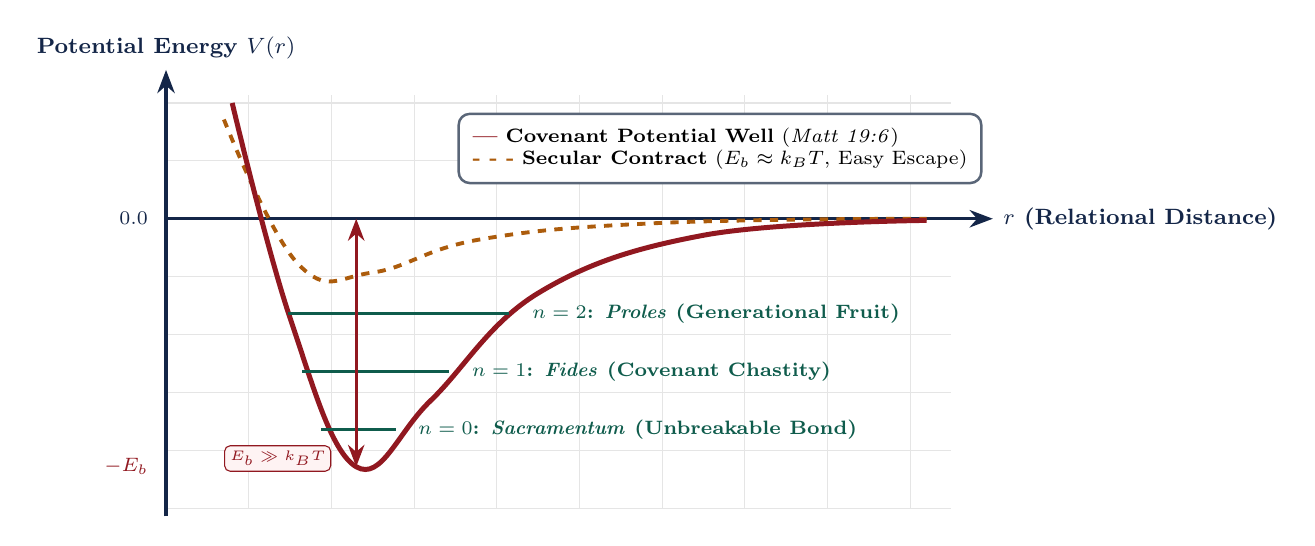
\begin{tikzpicture}[scale=1.05, >=Stealth]
  % Grid
  \draw[gray!20, thin] (0, -3.5) grid[xstep=1.0, ystep=0.7] (9.5, 1.5);

  % Axes
  \draw[->, line width=1.2pt, covenantblue] (0, 0) -- (10.0, 0) node[right, font=\footnotesize\bfseries, text=covenantblue] {$r$ (Relational Distance)};
  \draw[->, line width=1.2pt, covenantblue] (0, -3.6) -- (0, 1.8) node[above, font=\footnotesize\bfseries, text=covenantblue] {Potential Energy $V(r)$};

  % Zero Reference Label
  \node[left=3pt, font=\scriptsize\bfseries, text=covenantblue] at (0, 0) {$0.0$};
  \node[left=3pt, font=\scriptsize\bfseries, text=sacrificialred] at (0, -3.0) {$-E_b$};

  % Secular Shallow Curve (Dashed Amber)
  \draw[dashed, line width=1.4pt, filialamber]
    plot[smooth, tension=0.7] coordinates {(0.7, 1.2) (1.6, -0.55) (2.5, -0.65) (3.8, -0.25) (6.0, -0.05) (9.2, 0.0)};

  % Covenant Deep Morse-style Well (Solid Deep Red)
  \draw[line width=1.8pt, sacrificialred]
    plot[smooth, tension=0.65] coordinates {(0.8, 1.4) (1.5, -1.2) (2.3, -3.0) (3.2, -2.2) (4.5, -0.9) (6.5, -0.2) (9.2, -0.02)};

  % Quantized Bound Energy Levels inside Covenant Well
  \draw[line width=1.1pt, hearthteal] (1.88, -2.55) -- (2.78, -2.55);
  \node[right=4pt, font=\scriptsize\bfseries, text=hearthteal] at (2.8, -2.55) {$n=0$: \textit{Sacramentum} (Unbreakable Bond)};

  \draw[line width=1.1pt, hearthteal] (1.65, -1.85) -- (3.42, -1.85);
  \node[right=4pt, font=\scriptsize\bfseries, text=hearthteal] at (3.45, -1.85) {$n=1$: \textit{Fides} (Covenant Chastity)};

  \draw[line width=1.1pt, hearthteal] (1.48, -1.15) -- (4.15, -1.15);
  \node[right=4pt, font=\scriptsize\bfseries, text=hearthteal] at (4.18, -1.15) {$n=2$: \textit{Proles} (Generational Fruit)};

  % Binding Energy Double Arrow
  \draw[<->, line width=1.1pt, sacrificialred] (2.3, 0) -- (2.3, -3.0);
  \node[fill=sacrificialredfill, draw=sacrificialred, rounded corners=2pt, inner sep=2pt, font=\tiny\bfseries, text=sacrificialred] at (1.35, -2.9) {$E_b \gg k_B T$};

  % Legend Box in Upper Right
  \node[rectangle, rounded corners=4pt, draw=slateborder, fill=white, line width=0.9pt, inner sep=5pt, font=\scriptsize, align=left] at (6.7, 0.85) {
    \textcolor{sacrificialred}{\textbf{---}} \textbf{Covenant Potential Well} (\textit{Matt 19:6})\\
    \textcolor{filialamber}{\textbf{- - -}} \textbf{Secular Contract} ($E_b \approx k_B T$, Easy Escape)
  };
\end{tikzpicture}
\caption{\textbf{The Potential Energy Well of Sacred Matrimony.} St.~Augustine's \textit{tria bona} (\textit{sacramentum}, \textit{fides}, \textit{proles}) establish quantized bound states within a deep potential well ($E_b \gg k_B T$), preventing thermal dissociation during trials.}
\label{fig:potential_well}
\end{figure}

``In secular marriage,'' Feynman said, pointing to Figure~\ref{fig:potential_well}, ``people remove the \textit{sacramentum}. They flatten the potential well so that the binding energy is barely equal to room temperature ($E_b \approx k_B T$). The moment the temperature rises or an attractive external perturbation appears, the particle escapes! When marriage is sealed by covenant before God, the bond is indissoluble. It creates a deep potential well where children can grow in security.''

\chapter{The Classical Mechanics of Hierarchical Offices}

\section{The Hierarchy of Offices: God, Husband, Wife, Child}
Daniel leaned forward, studying his notes. ``Professor, modern culture recoils at the word \textit{hierarchy}. When people hear that the office of the husband is higher in hierarchy than the office of the wife, and that parents govern the children, they immediately think of tyranny. How does Christian patriarchy differ from authoritarian dominance?''

Feynman smiled, wiped his hands on his trousers, and drew a four-tier vertical structure on the center of the board (Figure~\ref{fig:textbook_hierarchy}).

``Let us look at structural mechanics, Daniel. In any complex assembly, such as a suspension bridge or a Saturn rocket, components have distinct load paths. Look at St.~Thomas Aquinas in the \textit{Summa Theologiae}, First Part, Question 92, Article 1. Aquinas distinguishes between two kinds of subjection:
\begin{enumerate}
    \item \textbf{Servile Subjection (\textit{servilis subjectio})}: Where a master rules a slave for the master's own private utility. That is tyranny!
    \item \textbf{Domestic Subjection (\textit{oeconomica subjectio})}: Where a leader directs free persons toward their own flourishing and the common good of the family.
\end{enumerate}
In the domestic church, the office of the husband stands strictly higher in hierarchy than the office of the wife under Christ, yet the wife is honored as a free queen consort and co-heir of grace!''

\begin{figure}[H]
\centering
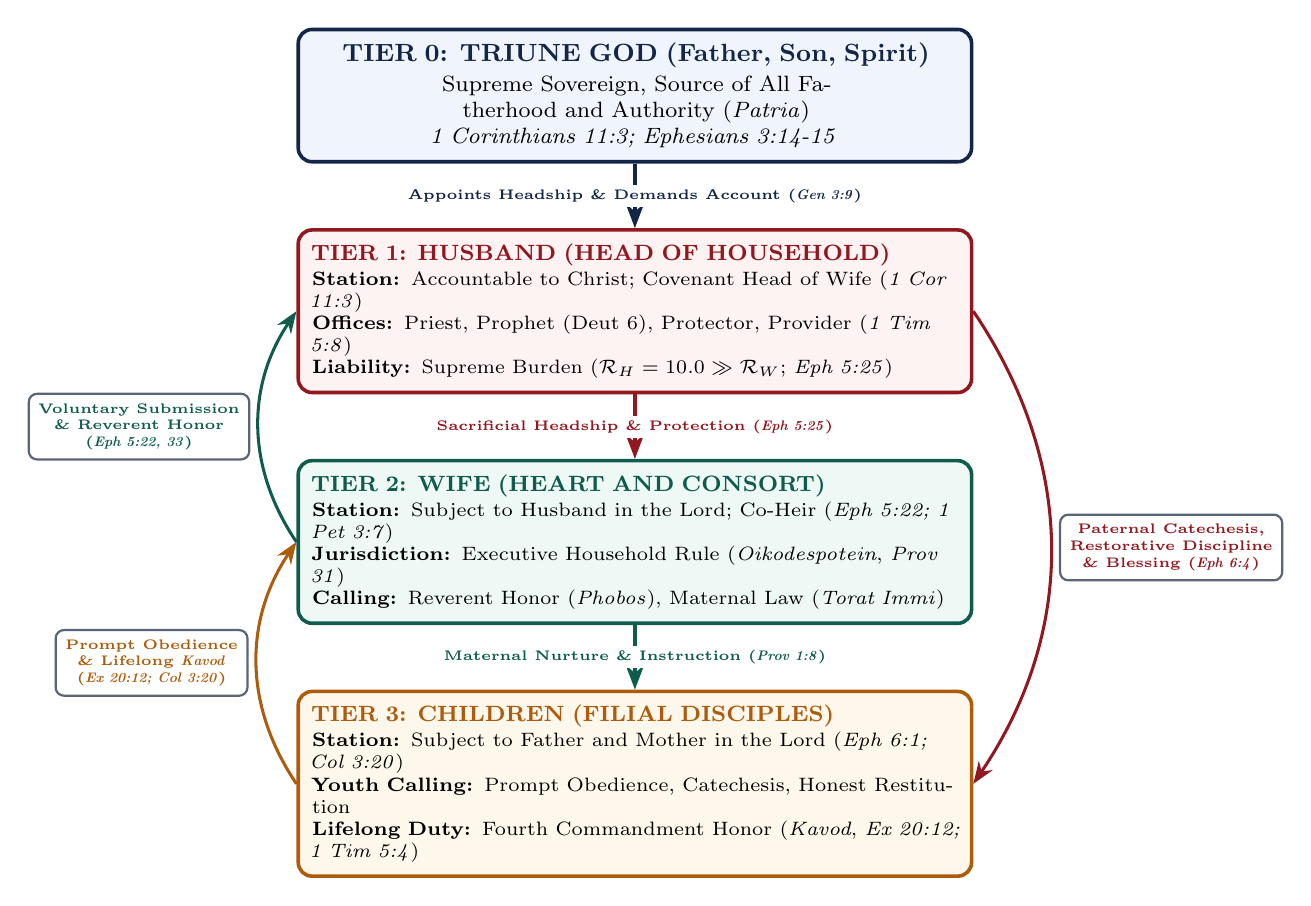
\begin{tikzpicture}[>=Stealth,
    headerbox/.style={rectangle, rounded corners=5pt, draw=covenantblue, line width=1.3pt, fill=covenantbluefill, text width=8.2cm, align=center, font=\footnotesize, inner sep=5pt},
    husbandbox/.style={rectangle, rounded corners=5pt, draw=sacrificialred, line width=1.3pt, fill=sacrificialredfill, text width=8.2cm, align=left, font=\scriptsize, inner sep=5pt},
    wifebox/.style={rectangle, rounded corners=5pt, draw=hearthteal, line width=1.3pt, fill=hearthtealfill, text width=8.2cm, align=left, font=\scriptsize, inner sep=5pt},
    childbox/.style={rectangle, rounded corners=5pt, draw=filialamber, line width=1.3pt, fill=filialamberfill, text width=8.2cm, align=left, font=\scriptsize, inner sep=5pt},
    sidebadge/.style={rectangle, rounded corners=3pt, draw=slateborder, line width=0.8pt, fill=white, font=\tiny\bfseries, align=center, inner sep=3.5pt}
]
  % Tier 0: Triune God
  \node[headerbox] (god) at (0, 6.8) {
    \textbf{\small\textcolor{covenantblue}{TIER 0: TRIUNE GOD (Father, Son, Spirit)}}\\[1pt]
    Supreme Sovereign, Source of All Fatherhood and Authority (\textit{Patria})\\
    \textit{1 Corinthians 11:3; Ephesians 3:14-15}
  };

  % Tier 1: Office of the Husband
  \node[husbandbox, below=0.82cm of god] (husband) {
    \textbf{\footnotesize\textcolor{sacrificialred}{TIER 1: HUSBAND (HEAD OF HOUSEHOLD)}}\\[1pt]
    \textbf{Station:} Accountable to Christ; Covenant Head of Wife (\textit{1 Cor 11:3})\\
    \textbf{Offices:} Priest, Prophet (Deut 6), Protector, Provider (\textit{1 Tim 5:8})\\
    \textbf{Liability:} Supreme Burden ($\mathcal{R}_H = 10.0 \gg \mathcal{R}_W$; \textit{Eph 5:25})
  };

  % Tier 2: Office of the Wife
  \node[wifebox, below=0.82cm of husband] (wife) {
    \textbf{\footnotesize\textcolor{hearthteal}{TIER 2: WIFE (HEART AND CONSORT)}}\\[1pt]
    \textbf{Station:} Subject to Husband in the Lord; Co-Heir (\textit{Eph 5:22; 1 Pet 3:7})\\
    \textbf{Jurisdiction:} Executive Household Rule (\textit{Oikodespotein}, \textit{Prov 31})\\
    \textbf{Calling:} Reverent Honor (\textit{Phobos}), Maternal Law (\textit{Torat Immi})
  };

  % Tier 3: Office of the Children
  \node[childbox, below=0.82cm of wife] (children) {
    \textbf{\footnotesize\textcolor{filialamber}{TIER 3: CHILDREN (FILIAL DISCIPLES)}}\\[1pt]
    \textbf{Station:} Subject to Father and Mother in the Lord (\textit{Eph 6:1; Col 3:20})\\
    \textbf{Youth Calling:} Prompt Obedience, Catechesis, Honest Restitution\\
    \textbf{Lifelong Duty:} Fourth Commandment Honor (\textit{Kavod}, \textit{Ex 20:12; 1 Tim 5:4})
  };

  % Downward Authority Arrows
  \draw[->, line width=1.3pt, covenantblue] (god.south) --
    node[midway, fill=white, inner sep=1.5pt, font=\tiny\bfseries, text=covenantblue] {Appoints Headship \& Demands Account (\textit{Gen 3:9})} (husband.north);

  \draw[->, line width=1.3pt, sacrificialred] (husband.south) --
    node[midway, fill=white, inner sep=1.5pt, font=\tiny\bfseries, text=sacrificialred] {Sacrificial Headship \& Protection (\textit{Eph 5:25})} (wife.north);

  \draw[->, line width=1.3pt, hearthteal] (wife.south) --
    node[midway, fill=white, inner sep=1.5pt, font=\tiny\bfseries, text=hearthteal] {Maternal Nurture \& Instruction (\textit{Prov 1:8})} (children.north);

  % Left Upward Honor Arcs
  \draw[->, line width=1.1pt, hearthteal] (wife.west) to[bend left=34]
    node[sidebadge, left=3pt] {Voluntary Submission\\\& Reverent Honor\\(\textit{Eph 5:22, 33})} (husband.west);

  \draw[->, line width=1.1pt, filialamber] (children.west) to[bend left=34]
    node[sidebadge, left=3pt] {Prompt Obedience\\\& Lifelong \textit{Kavod}\\(\textit{Ex 20:12; Col 3:20})} (wife.west);

  % Right Direct Paternal Governance Arc
  \draw[->, line width=1.1pt, sacrificialred] (husband.east) to[bend left=34]
    node[sidebadge, right=3pt] {Paternal Catechesis,\\Restorative Discipline\\\& Blessing (\textit{Eph 6:4})} (children.east);
\end{tikzpicture}
\caption{\textbf{The Four-Tier Vertical Hierarchy of the Covenant Household.} Authority flows downward from the Triune God through the Husband to the Wife and Children ($\text{God} \to \text{Husband} \to \text{Wife} \to \text{Children}$), while honor and obedience ascend upward.}
\label{fig:textbook_hierarchy}
\end{figure}

\section{The Principle of Inverse Proportionality}
Feynman wrote a bold formula on the chalkboard:
\begin{equation}
    \mathcal{R}_H \gg \mathcal{R}_W \gg \mathcal{R}_C
\end{equation}

``Here is the central law of Christian patriarchy, Daniel: \textbf{The Principle of Inverse Proportionality}. The severity of divine judgment and the burden of self-sacrifice strictly increase as you ascend the hierarchy!''

``In secular corporate hierarchies, the man at the top takes the bonuses and blames his subordinates when things go wrong,'' Daniel noted.

``Exactly! In the world, authority means entitlement. In the kingdom of Christ, authority means sacrifice! Christ declared in Mark 10:43-45: \textit{`Whoever would be great among you must be your servant, and whoever would be first among you must be slave of all.'}''

\begin{figure}[H]
\centering
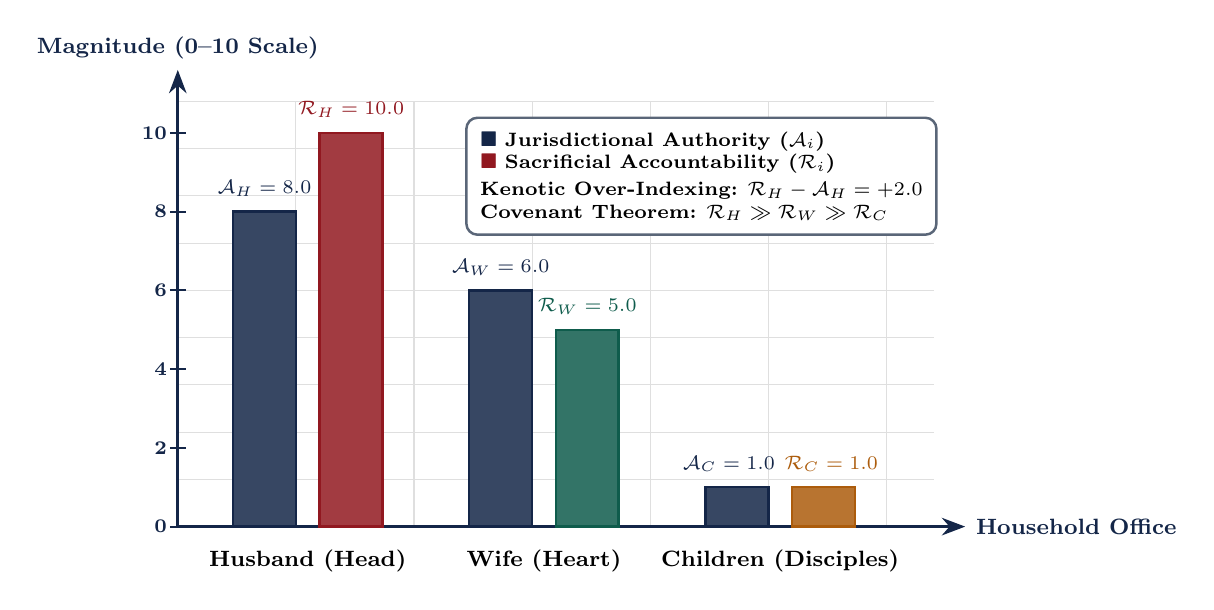
\begin{tikzpicture}[scale=1.0, >=Stealth]
  % Grid & Axes
  \draw[gray!25, thin] (0,0) grid[xstep=1.5, ystep=0.6] (9.6, 5.4);
  \draw[->, line width=1.2pt, covenantblue] (0,0) -- (10.0,0) node[right, font=\footnotesize\bfseries, text=covenantblue] {Household Office};
  \draw[->, line width=1.2pt, covenantblue] (0,0) -- (0,5.8) node[above, font=\footnotesize\bfseries, text=covenantblue] {Magnitude (0--10 Scale)};

  % Y-axis ticks
  \foreach \y/\val in {0/0, 1/2, 2/4, 3/6, 4/8, 5/10} {
    \draw[covenantblue, thick] (-0.1, \y) -- (0.1, \y) node[left=3pt, font=\scriptsize\bfseries] {\val};
  }

  % Husband Bars
  \fill[covenantblue!85, draw=covenantblue, line width=0.9pt] (0.7, 0) rectangle (1.5, 4.0);
  \node[above=2pt, font=\scriptsize\bfseries, text=covenantblue] at (1.1, 4.0) {$\mathcal{A}_H = 8.0$};

  \fill[sacrificialred!85, draw=sacrificialred, line width=0.9pt] (1.8, 0) rectangle (2.6, 5.0);
  \node[above=2pt, font=\scriptsize\bfseries, text=sacrificialred] at (2.2, 5.0) {$\mathcal{R}_H = 10.0$};
  \node[below=5pt, font=\footnotesize\bfseries] at (1.65, 0) {Husband (Head)};

  % Wife Bars
  \fill[covenantblue!85, draw=covenantblue, line width=0.9pt] (3.7, 0) rectangle (4.5, 3.0);
  \node[above=2pt, font=\scriptsize\bfseries, text=covenantblue] at (4.1, 3.0) {$\mathcal{A}_W = 6.0$};

  \fill[hearthteal!85, draw=hearthteal, line width=0.9pt] (4.8, 0) rectangle (5.6, 2.5);
  \node[above=2pt, font=\scriptsize\bfseries, text=hearthteal] at (5.2, 2.5) {$\mathcal{R}_W = 5.0$};
  \node[below=5pt, font=\footnotesize\bfseries] at (4.65, 0) {Wife (Heart)};

  % Children Bars
  \fill[covenantblue!85, draw=covenantblue, line width=0.9pt] (6.7, 0) rectangle (7.5, 0.5);
  \node[above=2pt, font=\scriptsize\bfseries, text=covenantblue] at (7.0, 0.5) {$\mathcal{A}_C = 1.0$};

  \fill[filialamber!85, draw=filialamber, line width=0.9pt] (7.8, 0) rectangle (8.6, 0.5);
  \node[above=2pt, font=\scriptsize\bfseries, text=filialamber] at (8.3, 0.5) {$\mathcal{R}_C = 1.0$};
  \node[below=5pt, font=\footnotesize\bfseries] at (7.65, 0) {Children (Disciples)};

  % Legend Box cleanly placed on upper right clear of R_H bar
  \node[rectangle, rounded corners=4pt, draw=slateborder, fill=white, line width=0.9pt, inner sep=5pt, font=\scriptsize, align=left] at (6.65, 4.45) {
    \textcolor{covenantblue}{$\blacksquare$} \textbf{Jurisdictional Authority ($\mathcal{A}_i$)}\\
    \textcolor{sacrificialred}{$\blacksquare$} \textbf{Sacrificial Accountability ($\mathcal{R}_i$)}\\[2pt]
    \textbf{Kenotic Over-Indexing:} $\mathcal{R}_H - \mathcal{A}_H = +2.0$\\
    \textbf{Covenant Theorem:} $\mathcal{R}_H \gg \mathcal{R}_W \gg \mathcal{R}_C$
  };
\end{tikzpicture}
\caption{\textbf{Quantitative Profile of the Responsibility Index.} The husband bears maximum sacrificial accountability ($\mathcal{R}_H = 10.0$), absorbing external hazards to shelter the wife and children.}
\label{fig:textbook_bars}
\end{figure}

Feynman tapped Figure~\ref{fig:textbook_bars} on the board. ``When Adam and Eve sinned in the garden, Eve ate the fruit first, yet when God walked into the garden in Genesis 3:9, He called out to Adam: \textit{`Where are you?'} As the covenant head, Adam was held accountable for the breach of his sanctuary. A Christian husband wakes up early, bears the weight of provision, shields his family from harm, and answers to God first.''

\chapter{The Coupled Oscillator: Holy Spouseship}

\section{The Husband as Head and the Wife as Heart}
``Now let us examine the magisterial encyclicals,'' Feynman said. ``Pope Leo XIII in \textit{Arcanum} (1880) and Pope Pius XI in \textit{Casti Connubii} (1930) provided an anatomical model of the family: \textbf{The husband is the head, and the wife is the heart}.''

``What happens in a living organism if the head tries to operate without the heart?'' Daniel asked.

``The body perishes!'' Feynman exclaimed. ``A man who governs his home without the warm, perceptive wisdom of his wife turns his household into a cold barracks. And if the heart tries to usurp the head, the home loses structural direction.''

\section{The Wife's Executive Calling: Proverbs 31 and Oikodespotein}
``Look at Proverbs 31:10-31,'' Feynman said. ``She inspects a field and buys it with her earnings; she plants a vineyard; she directs her household; she opens her mouth with wisdom and the teaching of kindness is on her tongue! St.~Paul uses the Greek verb \textit{oikodespotein} in 1 Timothy 5:14, which literally means \textit{to rule the household} as its domestic executive!''

\begin{blackboard}
\textbf{The Symmetrical Complementarity of Holy Spouseship:}
\begin{itemize}
    \item \textbf{Husband (Head)}: Outer Perimeter Defense, Economic Sustenance, Sacrificial Headship, Spiritual Priesthood (\textit{Eph 5:23-29; 1 Tim 5:8}).
    \item \textbf{Wife (Heart)}: Interior Sanctuary Governance, Relational Nurture, Executive Household Management, Reverent Honor (\textit{Prov 31:10-31; 1 Tim 5:14}).
\end{itemize}
\end{blackboard}

\section{The Casuistry of Peace: Richard Baxter's Rules}
``Puritan divine Richard Baxter, in \textit{A Christian Directory} (1673), gave practical rules for married couples that every physicist should appreciate,'' Feynman said:
\begin{enumerate}
    \item Remember that you are both fallen human beings with infirmities; resolve to bear patiently with each other's weaknesses.
    \item Agree beforehand that when one spouse is overtaken by frustration, the other will remain calm and speak with gentle softness until peace returns.
    \item Settle every disagreement before sleep: never let the sun go down upon your anger (Ephesians 4:26).
\end{enumerate}

``Marriage operates like a coupled mechanical harmonic oscillator with a viscous dashpot damper,'' Feynman said, sketching Figure~\ref{fig:coupled_oscillator}. ``The spring constant $k_c$ is the unbreakable covenant bond of vows. The dashpot damper $c_d$ is forgiving grace and mutual forbearance. When an external shock hits one spouse, the damper dissipates the kinetic energy of anger into harmless heat before destructive resonance can tear the system apart!''

\begin{figure}[H]
\centering
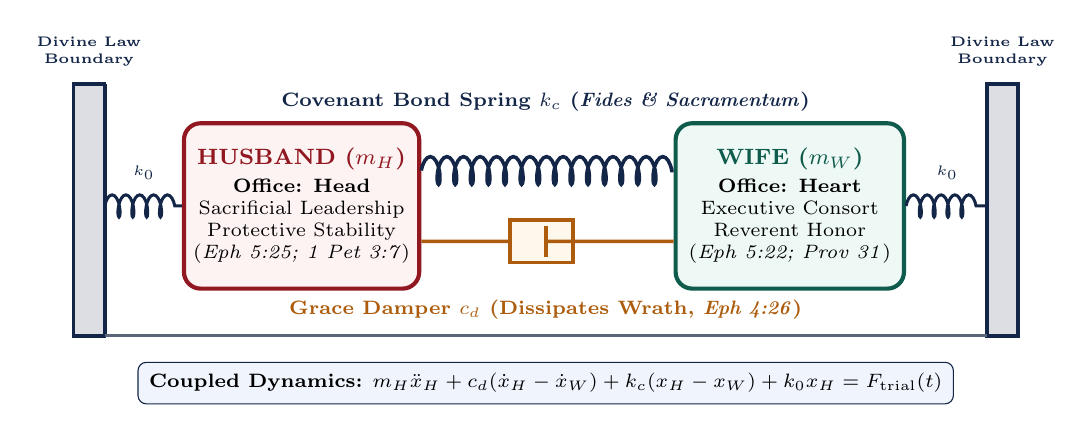
\begin{tikzpicture}[scale=1.0, >=Stealth,
    wall/.style={fill=covenantblue!15, draw=covenantblue, line width=1.2pt},
    massH/.style={rectangle, rounded corners=6pt, draw=sacrificialred, line width=1.5pt, fill=sacrificialredfill, minimum width=2.9cm, minimum height=2.1cm, align=center, font=\scriptsize},
    massW/.style={rectangle, rounded corners=6pt, draw=hearthteal, line width=1.5pt, fill=hearthtealfill, minimum width=2.9cm, minimum height=2.1cm, align=center, font=\scriptsize}
]
  % Left & Right Boundary Walls (God's Law)
  \fill[wall] (-6.0, -1.65) rectangle (-5.6, 1.55);
  \draw[line width=1.4pt, covenantblue] (-5.6, -1.65) -- (-5.6, 1.55);
  \node[above=3pt, font=\tiny\bfseries, text=covenantblue, align=center] at (-5.8, 1.55) {Divine Law\\Boundary};

  \fill[wall] (5.6, -1.65) rectangle (6.0, 1.55);
  \draw[line width=1.4pt, covenantblue] (5.6, -1.65) -- (5.6, 1.55);
  \node[above=3pt, font=\tiny\bfseries, text=covenantblue, align=center] at (5.8, 1.55) {Divine Law\\Boundary};

  % Floor Track
  \draw[line width=1.1pt, slateborder] (-5.6, -1.65) -- (5.6, -1.65);

  % Husband Mass (Left)
  \node[massH] (mH) at (-3.1, 0.0) {
    \textbf{\footnotesize\textcolor{sacrificialred}{HUSBAND ($m_H$)}}\\[2pt]
    \textbf{Office: Head}\\
    Sacrificial Leadership\\
    Protective Stability\\
    (\textit{Eph 5:25; 1 Pet 3:7})
  };

  % Wife Mass (Right)
  \node[massW] (mW) at (3.1, 0.0) {
    \textbf{\footnotesize\textcolor{hearthteal}{WIFE ($m_W$)}}\\[2pt]
    \textbf{Office: Heart}\\
    Executive Consort\\
    Reverent Honor\\
    (\textit{Eph 5:22; Prov 31})
  };

  % Outer Anchoring Springs to Divine Law
  \draw[decoration={aspect=0.35, segment length=5pt, amplitude=4pt, coil}, decorate, line width=1.1pt, covenantblue] (-5.6, 0) -- (mH.west);
  \node[above=6pt, font=\tiny\bfseries, text=covenantblue] at (-5.1, 0) {$k_0$};

  \draw[decoration={aspect=0.35, segment length=5pt, amplitude=4pt, coil}, decorate, line width=1.1pt, covenantblue] (mW.east) -- (5.6, 0);
  \node[above=6pt, font=\tiny\bfseries, text=covenantblue] at (5.1, 0) {$k_0$};

  % Top Coupling Spring k_c (Covenant Vows)
  \draw[decoration={aspect=0.35, segment length=6pt, amplitude=5pt, coil}, decorate, line width=1.3pt, covenantblue]
    ([yshift=0.45cm]mH.east) -- ([yshift=0.45cm]mW.west);
  \node[font=\scriptsize\bfseries, text=covenantblue] at (0, 1.32) {Covenant Bond Spring $k_c$ (\textit{Fides \& Sacramentum})};

  % Bottom Dashpot Damper c_d (Forgiveness & Grace)
  \draw[line width=1.3pt, filialamber] ([yshift=-0.45cm]mH.east) -- (-0.45, -0.45);
  \draw[line width=1.3pt, filialamber, fill=filialamberfill] (-0.45, -0.72) rectangle (0.35, -0.18);
  \draw[line width=1.5pt, filialamber] (0.0, -0.65) -- (0.0, -0.25);
  \draw[line width=1.3pt, filialamber] (0.0, -0.45) -- ([yshift=-0.45cm]mW.west);
  \node[font=\scriptsize\bfseries, text=filialamber] at (0, -1.32) {Grace Damper $c_d$ (Dissipates Wrath, \textit{Eph 4:26})};

  % Equation Box Below
  \node[rectangle, rounded corners=3pt, draw=covenantblue, fill=covenantbluefill, inner sep=4pt, font=\scriptsize] at (0, -2.25) {
    \textbf{Coupled Dynamics:} $m_H \ddot{x}_H + c_d(\dot{x}_H - \dot{x}_W) + k_c(x_H - x_W) + k_0 x_H = F_{\text{trial}}(t)$
  };
\end{tikzpicture}
\caption{\textbf{The Coupled Harmonic Oscillator Model of Holy Spouseship.} The covenant spring $k_c$ binds husband and wife in one-flesh unity, while the viscous dashpot damper $c_d$ (forgiving grace and patience) absorbs external shocks and prevents destructive resonance.}
\label{fig:coupled_oscillator}
\end{figure}

\chapter{Paternal Mechanics: Torque, Boundaries, and Catechesis}

\section{The Father's Office: The Deuteronomy 6 Liturgy}
Feynman stood in front of the board, drawing a 24-hour compass rose with four cardinal stations: Rising at Dawn, Walking by the Way, Sitting at the Table, and Lying Down at Night (Figure~\ref{fig:circadian_liturgy}).

``Now, Daniel, let us talk about parenting. Look at Deuteronomy 6:6-7: \textit{`These words that I command you today shall be on your heart. You shall teach them diligently to your children, and shall talk of them when you sit in your house, and when you walk by the way, and when you lie down, and when you rise.'} God placed primary catechetical responsibility directly on the father! The home is the primary laboratory of truth.''

\begin{figure}[H]
\centering
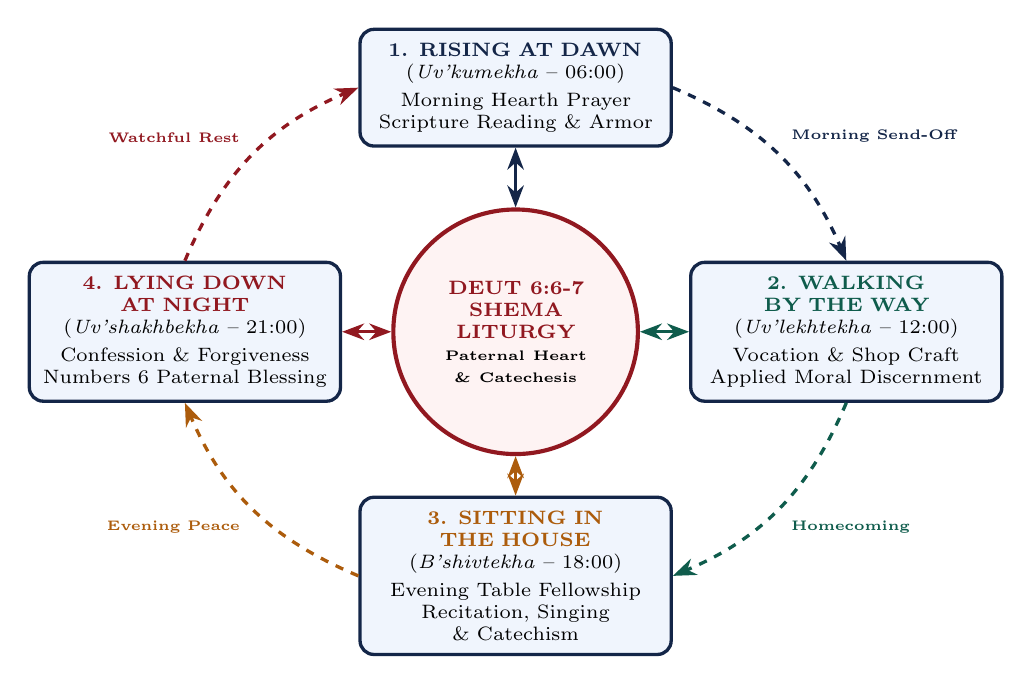
\begin{tikzpicture}[scale=1.0, >=Stealth,
    station/.style={rectangle, rounded corners=5pt, draw=covenantblue, line width=1.2pt, fill=covenantbluefill, text width=3.6cm, align=center, font=\scriptsize, inner sep=5pt},
    hub/.style={circle, draw=sacrificialred, line width=1.5pt, fill=sacrificialredfill, text width=2.4cm, align=center, font=\scriptsize\bfseries, inner sep=4pt}
]
  % Central Hub
  \node[hub] (center) at (0,0) {
    \textcolor{sacrificialred}{DEUT 6:6-7}\\
    \textcolor{sacrificialred}{SHEMA}\\
    \textcolor{sacrificialred}{LITURGY}\\[2pt]
    \tiny Paternal Heart\\\& Catechesis
  };

  % 4 Cardinal Stations
  \node[station] (north) at (0, 3.1) {
    \textbf{\textcolor{covenantblue}{1. RISING AT DAWN}}\\
    (\textit{Uv'kumekha} -- 06:00)\\[2pt]
    Morning Hearth Prayer\\
    Scripture Reading \& Armor
  };

  \node[station] (east) at (4.2, 0) {
    \textbf{\textcolor{hearthteal}{2. WALKING BY THE WAY}}\\
    (\textit{Uv'lekhtekha} -- 12:00)\\[2pt]
    Vocation \& Shop Craft\\
    Applied Moral Discernment
  };

  \node[station] (south) at (0, -3.1) {
    \textbf{\textcolor{filialamber}{3. SITTING IN THE HOUSE}}\\
    (\textit{B'shivtekha} -- 18:00)\\[2pt]
    Evening Table Fellowship\\
    Recitation, Singing \& Catechism
  };

  \node[station] (west) at (-4.2, 0) {
    \textbf{\textcolor{sacrificialred}{4. LYING DOWN AT NIGHT}}\\
    (\textit{Uv'shakhbekha} -- 21:00)\\[2pt]
    Confession \& Forgiveness\\
    Numbers 6 Paternal Blessing
  };

  % Connecting Spokes
  \draw[<->, line width=1.1pt, covenantblue] (center.north) -- (north.south);
  \draw[<->, line width=1.1pt, hearthteal] (center.east) -- (east.west);
  \draw[<->, line width=1.1pt, filialamber] (center.south) -- (south.north);
  \draw[<->, line width=1.1pt, sacrificialred] (center.west) -- (west.east);

  % Clockwise Circadian Cycle Arrows
  \draw[->, line width=1.2pt, dashed, covenantblue] (north.east) to[bend left=22]
    node[midway, above right=1pt, font=\tiny\bfseries, text=covenantblue] {Morning Send-Off} (east.north);

  \draw[->, line width=1.2pt, dashed, hearthteal] (east.south) to[bend left=22]
    node[midway, below right=1pt, font=\tiny\bfseries, text=hearthteal] {Homecoming} (south.east);

  \draw[->, line width=1.2pt, dashed, filialamber] (south.west) to[bend left=22]
    node[midway, below left=1pt, font=\tiny\bfseries, text=filialamber] {Evening Peace} (west.south);

  \draw[->, line width=1.2pt, dashed, sacrificialred] (west.north) to[bend left=22]
    node[midway, above left=1pt, font=\tiny\bfseries, text=sacrificialred] {Watchful Rest} (north.west);
\end{tikzpicture}
\caption{\textbf{The Circadian Liturgy of Paternal Catechesis (Deuteronomy 6:6-7).} Spiritual formation operates as a continuous 24-hour cycle anchored by the father's presence at dawn, midday labor, supper table, and bedtime blessing.}
\label{fig:circadian_liturgy}
\end{figure}

\section{Ephesians 6:4: Non-Provocation and Restorative Discipline}
``Look at Ephesians 6:4,'' Feynman continued. ``\textit{`Fathers, do not provoke your children to anger, but bring them up in the discipline and instruction of the Lord.'} And Colossians 3:21: \textit{`Fathers, do not provoke your children, lest they become discouraged.'}''

``How does a father discipline effectively without provoking a child to anger or using harshness, Professor?''

``By obeying the laws of stable control systems!'' Feynman said:
\begin{itemize}
    \item \textbf{Zero Hysteresis (Consistency)}: Never laugh at a transgression on Monday and explode in anger over the same act on Tuesday.
    \item \textbf{Moral Clarity Over Fury}: Address the conscience with calm, sorrowful gravity. Expose falsehood with truth (Proverbs 12:22).
    \item \textbf{Restitution Through Honest Labor}: If a child breaks property or breaches trust, require real restitution through work and temporary forfeiture of privileges (Exodus 22:14) until the debt is paid and fellowship is restored.
\end{itemize}

\chapter{Maternal Thermodynamics: Emotional Nurture and Affection}

\section{The Mother's Law: Torat Immi}
``What about the mother's office in child rearing?'' Daniel asked.

Feynman's voice softened. ``In Proverbs 1:8, Solomon writes: \textit{`Hear, my son, your father's instruction, and forsake not your mother's teaching (torat immi).'} The mother's law is the law of loving affection, relational warmth, and the moral conscience. A father erects the structural timbers of the house; the mother fills the house with warmth, beauty, and life-giving comfort (Isaiah 66:13).''

\begin{figure}[H]
\centering
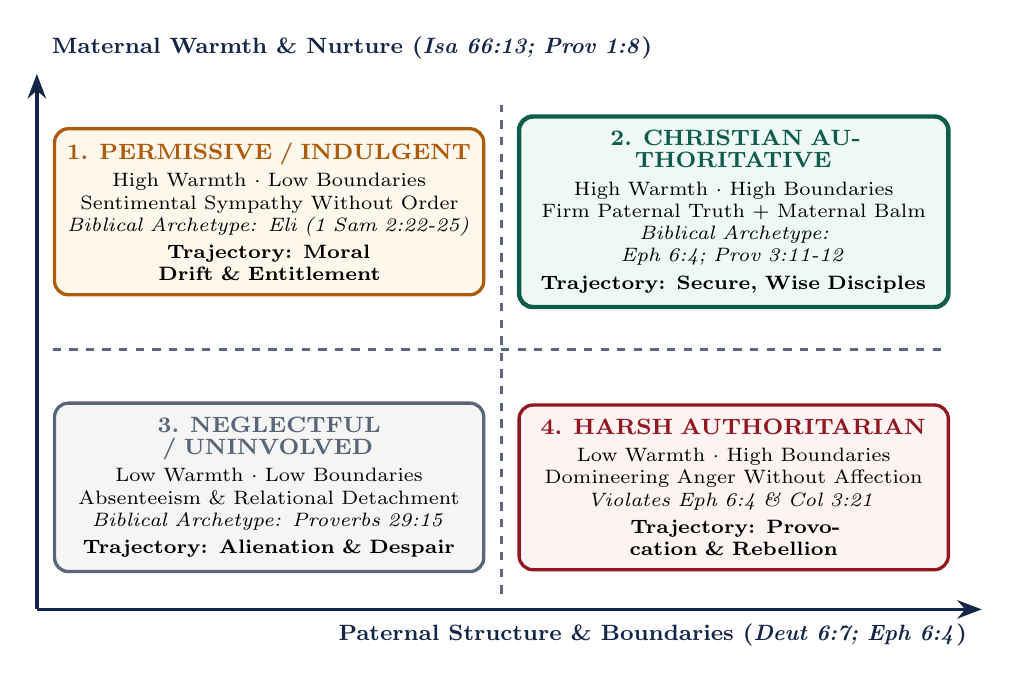
\begin{tikzpicture}[scale=1.0, >=Stealth,
    qbox/.style={rectangle, rounded corners=5pt, line width=1.2pt, text width=5.1cm, minimum height=2.0cm, align=center, font=\scriptsize, inner sep=5pt}
]
  % Axes
  \draw[->, line width=1.3pt, covenantblue] (0,0) -- (12.0,0) node[below left=2pt, font=\footnotesize\bfseries, text=covenantblue] {Paternal Structure \& Boundaries (\textit{Deut 6:7; Eph 6:4})};
  \draw[->, line width=1.3pt, covenantblue] (0,0) -- (0,6.8) node[above right=2pt, font=\footnotesize\bfseries, text=covenantblue] {Maternal Warmth \& Nurture (\textit{Isa 66:13; Prov 1:8})};

  % Quadrant 1: Permissive (Top Left)
  \node[qbox, draw=filialamber, fill=filialamberfill] at (2.95, 5.05) {
    \textbf{\footnotesize\textcolor{filialamber}{1. PERMISSIVE / INDULGENT}}\\[2pt]
    High Warmth $\cdot$ Low Boundaries\\
    Sentimental Sympathy Without Order\\
    \textit{Biblical Archetype: Eli (1 Sam 2:22-25)}\\[2pt]
    \textbf{Trajectory: Moral Drift \& Entitlement}
  };

  % Quadrant 2: Christian Authoritative (Top Right)
  \node[qbox, draw=hearthteal, line width=1.6pt, fill=hearthtealfill] at (8.85, 5.05) {
    \textbf{\footnotesize\textcolor{hearthteal}{2. CHRISTIAN AUTHORITATIVE}}\\[2pt]
    High Warmth $\cdot$ High Boundaries\\
    Firm Paternal Truth + Maternal Balm\\
    \textit{Biblical Archetype: Eph 6:4; Prov 3:11-12}\\[2pt]
    \textbf{Trajectory: Secure, Wise Disciples}
  };

  % Quadrant 3: Neglectful (Bottom Left)
  \node[qbox, draw=slateborder, fill=gray!8] at (2.95, 1.55) {
    \textbf{\footnotesize\textcolor{slateborder}{3. NEGLECTFUL / UNINVOLVED}}\\[2pt]
    Low Warmth $\cdot$ Low Boundaries\\
    Absenteeism \& Relational Detachment\\
    \textit{Biblical Archetype: Proverbs 29:15}\\[2pt]
    \textbf{Trajectory: Alienation \& Despair}
  };

  % Quadrant 4: Authoritarian (Bottom Right)
  \node[qbox, draw=sacrificialred, fill=sacrificialredfill] at (8.85, 1.55) {
    \textbf{\footnotesize\textcolor{sacrificialred}{4. HARSH AUTHORITARIAN}}\\[2pt]
    Low Warmth $\cdot$ High Boundaries\\
    Domineering Anger Without Affection\\
    \textit{Violates Eph 6:4 \& Col 3:21}\\[2pt]
    \textbf{Trajectory: Provocation \& Rebellion}
  };

  % Center Dividers cleanly in the gaps
  \draw[dashed, line width=1.0pt, covenantblue!70] (5.9, 0.2) -- (5.9, 6.4);
  \draw[dashed, line width=1.0pt, covenantblue!70] (0.2, 3.3) -- (11.5, 3.3);
\end{tikzpicture}
\caption{\textbf{The Christian Authoritative Parenting Matrix.} Synthesizing high paternal moral structure with high maternal warmth produces secure, virtuous disciples while avoiding authoritarian provocation and permissive drift.}
\label{fig:textbook_parenting}
\end{figure}

\section{The Unified Parental Front}
``Never allow a seam between father and mother,'' Feynman warned, pointing to Figure~\ref{fig:textbook_parenting}. ``Parents must confer in private, maintain solidarity in public, and uphold each other's honor before the children. When paternal correction is followed immediately by maternal comfort and encouragement, the child experiences both the holiness and the mercy of God.''

\chapter{The Fourth Commandment: Generational Conservation Laws}

\section{Honor (Kavod) as a Universal Conservation Principle}
``Finally, Daniel, look at Exodus 20:12: \textit{`Honor your father and your mother, that your days may be long in the land that the Lord your God is giving you.'}''

Feynman wrote on the board:
\begin{blackboard}
\centering
\Large \textbf{\textit{Kavod}} (Hebrew: \textit{kavod}) = Weight, Gravity, Reverent Honor
\end{blackboard}

``In Hebrew, honor is \textit{kavod}, meaning weighty, possessing gravitational mass! To dishonor a parent is to treat them as light (\textit{qalal}), negligible, disposable. St.~Thomas Aquinas placed the Fourth Commandment under the virtue of justice (\textit{pietas}, \textit{Summa Theologiae} II-II, q. 101). After God, your parents gave you life, fed you in infancy, and sheltered your youth. You owe them a lifelong debt of gratitude.''

\section{The Two Phases of the Fourth Commandment}
``The Fourth Commandment operates across two distinct phases of the human lifespan (Figure~\ref{fig:kavod_timeline}):
\begin{enumerate}
    \item \textbf{Phase I: Childhood and Youth (Direct Obedience)}: \textit{`Children, obey your parents in everything, for this pleases the Lord'} (Colossians 3:20; Ephesians 6:1).
    \item \textbf{Phase II: Adulthood (Lifelong Honor and Elder Care)}: When a man or woman marries (Genesis 2:24), a new household jurisdiction is formed. Direct parental command ceases, yet the obligation of \textit{kavod} intensifies! Adult children must honor their aging parents, seek their wisdom, and provide material and domestic shelter when their strength fails (1 Timothy 5:4, 8; Sirach 3:12-14).''
\end{enumerate}

\begin{figure}[H]
\centering
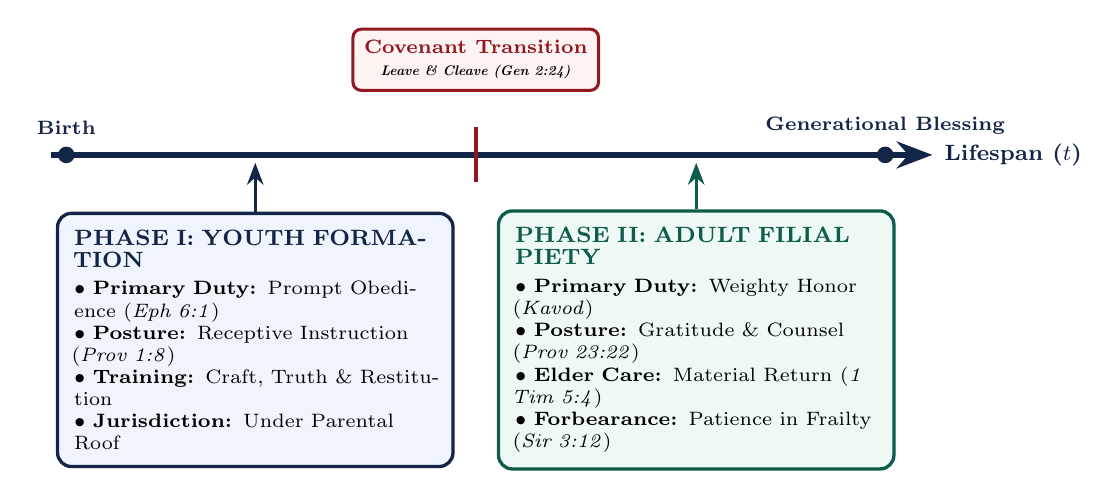
\begin{tikzpicture}[scale=1.0, >=Stealth,
    phasebox/.style={rectangle, rounded corners=5pt, line width=1.2pt, text width=4.6cm, align=left, font=\scriptsize, inner sep=6pt},
    milestone/.style={rectangle, rounded corners=3pt, draw=sacrificialred, line width=1.1pt, fill=sacrificialredfill, font=\scriptsize\bfseries, align=center, inner sep=4pt}
]
  % Main Lifespan Axis
  \draw[->, line width=2.2pt, covenantblue] (0, 0) -- (11.2, 0) node[right, font=\footnotesize\bfseries, text=covenantblue] {Lifespan ($t$)};

  % Phase Divider Tick at x = 5.4
  \draw[line width=1.6pt, sacrificialred] (5.4, -0.35) -- (5.4, 0.35);
  \node[milestone, above=0.45cm] at (5.4, 0.35) {
    \textcolor{sacrificialred}{Covenant Transition}\\
    \tiny \textit{Leave \& Cleave (Gen 2:24)}
  };

  % Start & End Ticks
  \fill[covenantblue] (0.2, 0) circle (3pt) node[above=4pt, font=\scriptsize\bfseries] {Birth};
  \fill[covenantblue] (10.6, 0) circle (3pt) node[above=4pt, font=\scriptsize\bfseries] {Generational Blessing};

  % Phase 1 Box (Below Left)
  \node[phasebox, draw=covenantblue, fill=covenantbluefill] (p1) at (2.6, -2.35) {
    \textbf{\footnotesize\textcolor{covenantblue}{PHASE I: YOUTH FORMATION}}\\[2pt]
    $\bullet$ \textbf{Primary Duty:} Prompt Obedience (\textit{Eph 6:1})\\
    $\bullet$ \textbf{Posture:} Receptive Instruction (\textit{Prov 1:8})\\
    $\bullet$ \textbf{Training:} Craft, Truth \& Restitution\\
    $\bullet$ \textbf{Jurisdiction:} Under Parental Roof
  };

  % Phase 2 Box (Below Right)
  \node[phasebox, draw=hearthteal, fill=hearthtealfill] (p2) at (8.2, -2.35) {
    \textbf{\footnotesize\textcolor{hearthteal}{PHASE II: ADULT FILIAL PIETY}}\\[2pt]
    $\bullet$ \textbf{Primary Duty:} Weighty Honor (\textit{Kavod})\\
    $\bullet$ \textbf{Posture:} Gratitude \& Counsel (\textit{Prov 23:22})\\
    $\bullet$ \textbf{Elder Care:} Material Return (\textit{1 Tim 5:4})\\
    $\bullet$ \textbf{Forbearance:} Patience in Frailty (\textit{Sir 3:12})
  };

  % Braces / Connectors to Timeline
  \draw[<-, line width=1.1pt, covenantblue] (2.6, -0.1) -- (p1.north);
  \draw[<-, line width=1.1pt, hearthteal] (8.2, -0.1) -- (p2.north);
\end{tikzpicture}
\caption{\textbf{The Two-Phase Lifecycle of the Fourth Commandment (\textit{Exodus 20:12}).} While Genesis 2:24 transitions a child from direct domestic obedience to autonomous household governance upon marriage, the duty of weighty honor (\textit{kavod}) and elder care endures across the entire lifespan.}
\label{fig:kavod_timeline}
\end{figure}

\chapter{Homework Problem Sets and Solutions}

\section{Problem Set 1: Mechanics of Spousal Order}

\subsection*{Problem 1.1: The Asymmetric Career Offer}
Daniel is offered a supervisory railway contract that increases his income substantially, but requires him to lodge away from home five days a week. His wife, Nora, points out that sixteen-year-old Hannah is on the threshold of womanhood, ten-year-old Caleb needs daily paternal guidance, and Daniel's aging father Thomas requires physical assistance after his stroke.
\begin{enumerate}
    \item Formulate the decision using the Responsibility Index ($\mathcal{R}_H \gg \mathcal{R}_W$).
    \item Evaluate whether accepting the contract fulfills 1 Timothy 5:8 or violates Ephesians 6:4 and Deuteronomy 6:6-7.
    \item Provide the optimal covenantal resolution.
\end{enumerate}

\begin{blackboard}
\textbf{Solution to Problem 1.1:}
\begin{enumerate}
    \item \textit{Responsibility Calculus}: The husband holds primary accountability $\mathcal{R}_H = 10.0$ before God for the spiritual protection, daily catechesis, and stability of his household. Financial gain beyond sufficiency cannot substitute for paternal presence.
    \item \textit{Scriptural Evaluation}: While 1 Timothy 5:8 commands material provision, Deuteronomy 6:6-7 and Ephesians 6:4 mandate daily circadian instruction and oversight. Trading five days a week of paternal headship for surplus gold leaves the wife overburdened and the children unguarded.
    \item \textit{Resolution}: Listen to the wise counsel of the wife (\textit{ezer kenegdo}), decline the distant contract, accept tighter financial margins locally, and preserve the daily integrity of the domestic church.
\end{enumerate}
\end{blackboard}

\section{Problem Set 2: Child Discipline and Paternal Restraint}

\subsection*{Problem 2.1: The Smashed Heirloom}
Ten-year-old Caleb disobeys household rules by throwing an ash stick indoors, shatters an heirloom brass lantern chimney, and lies to his parents by claiming the wind blew the window open.
\begin{enumerate}
    \item Diagnose the relative severity of the offenses (property damage vs. breach of truth).
    \item Design a real, non-physical authoritative disciplinary response that upholds Ephesians 6:4.
    \item Map the transition from paternal correction to maternal comfort and restoration.
\end{enumerate}

\begin{blackboard}
\textbf{Solution to Problem 2.1:}
\begin{enumerate}
    \item \textit{Diagnosis}: A broken glass chimney is replaceable material property; a deliberate lie to parents breaches the covenant of trust (Proverbs 12:22). The moral falsehood is the primary spiritual crisis.
    \item \textit{Paternal Correction (Non-Physical and Restorative)}: The father remains completely calm, exposing the falsehood through objective facts (the latched window). Without shouting or physical strikes, he brings the boy to genuine repentance and assigns full restitution: working Saturday afternoon in the machine shop sorting scrap iron and turning brass stock to earn the price of a new chimney (Exodus 22:14), alongside forfeiture of evening leisure.
    \item \textit{Maternal Balm}: Once confession is made and the restitution sentence accepted, the mother embraces the repentant boy, assures him of his cherished status as a beloved son (Hebrews 12:6-8), and works alongside him and his sister Hannah to clean the hearth rug.
\end{enumerate}
\end{blackboard}

\chapter{Examinations and Solutions}

\section{Midterm Examination}

\subsection*{Question 1: The Three Goods and Game-Theoretic Equilibrium}
Contrast St.~Augustine's \textit{tria bona} (\textit{proles}, \textit{fides}, \textit{sacramentum}) with the modern secular model of no-fault contractual marriage using extensive-form game theory.

\begin{blackboard}
\textbf{Midterm Solution 1:}
Under St.~Augustine's \textit{tria bona}, marriage is an objective covenantal reality sealed before God. In secular contractualism, payoffs follow a Prisoner's Dilemma ($T = 5 > R = 3 > P = 0 > S_0 = -3$), driving self-protective spouses into bilateral defection $(D,D)$. In covenantal marriage, divine accountability ($\theta_i > T - R$) and sanctification grace ($\gamma_i > 0$) transform the payoff matrix so that mutual sacrificial love $(S,S)$ is the strictly dominant, subgame-perfect Nash equilibrium.
\end{blackboard}

\section{Final Comprehensive Examination}

\subsection*{Case Study: The Crisis of Elder Care}
Daniel's elderly father, Thomas, suffers from post-stroke memory confusion. An acquaintance suggests placing Thomas in a distant institutional facility so Daniel can expand shop production.
\begin{enumerate}
    \item Analyze this proposal under the Fourth Commandment (Exodus 20:12), 1 Timothy 5:4-8, and Sirach 3:12-14.
    \item Explain how Daniel's care for his father models filial piety for sixteen-year-old Hannah and ten-year-old Caleb.
    \item Trace the operational protocol in Figure~\ref{fig:elder_protocol}.
\end{enumerate}

\begin{figure}[H]
\centering
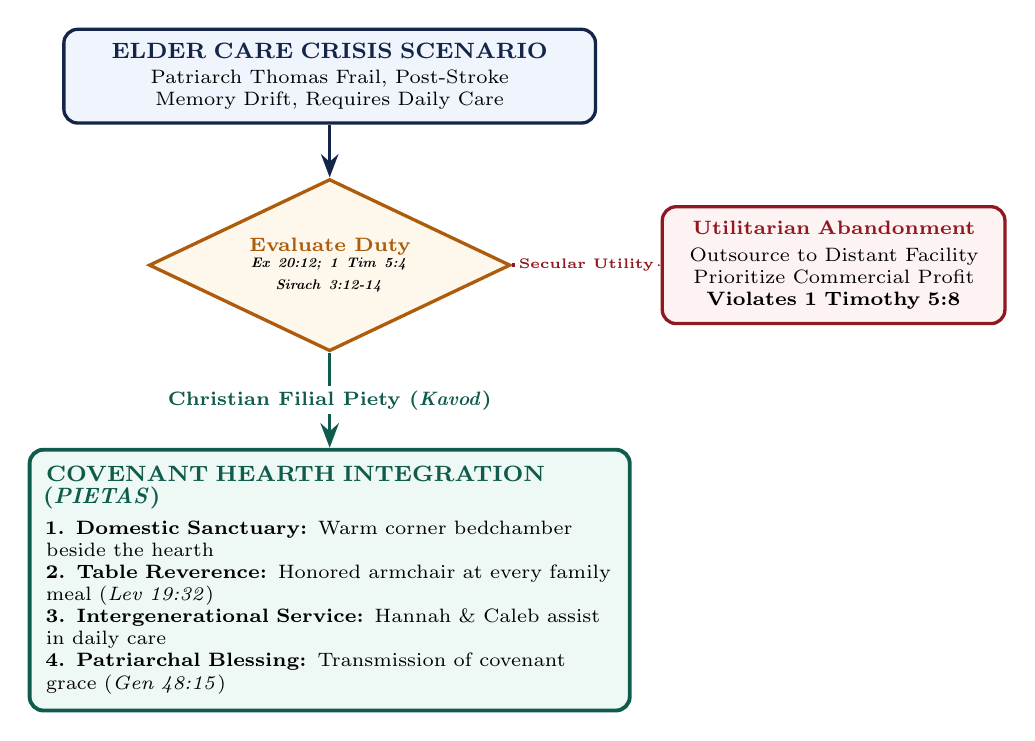
\begin{tikzpicture}[scale=1.0, >=Stealth,
    triggerbox/.style={rectangle, rounded corners=5pt, draw=covenantblue, line width=1.2pt, fill=covenantbluefill, text width=6.4cm, align=center, font=\scriptsize, inner sep=5pt},
    decbox/.style={diamond, aspect=2.1, draw=filialamber, line width=1.2pt, fill=filialamberfill, text width=2.8cm, align=center, font=\scriptsize\bfseries, inner sep=1.5pt},
    rejectbox/.style={rectangle, rounded corners=5pt, draw=sacrificialred, line width=1.2pt, fill=sacrificialredfill, text width=4.0cm, align=center, font=\scriptsize, inner sep=5pt},
    covenantbox/.style={rectangle, rounded corners=5pt, draw=hearthteal, line width=1.4pt, fill=hearthtealfill, text width=7.2cm, align=left, font=\scriptsize, inner sep=6pt}
]
  % Top Trigger Node
  \node[triggerbox] (trigger) at (0, 4.7) {
    \textbf{\footnotesize\textcolor{covenantblue}{ELDER CARE CRISIS SCENARIO}}\\[1pt]
    Patriarch Thomas Frail, Post-Stroke Memory Drift, Requires Daily Care
  };

  % Decision Diamond
  \node[decbox] (decide) at (0, 2.3) {
    \textcolor{filialamber}{Evaluate Duty}\\
    \tiny \textit{Ex 20:12; 1 Tim 5:4}\\
    \tiny \textit{Sirach 3:12-14}
  };

  % Secular Branch (Right)
  \node[rejectbox] (secular) at (6.4, 2.3) {
    \textbf{\textcolor{sacrificialred}{Utilitarian Abandonment}}\\[2pt]
    Outsource to Distant Facility\\
    Prioritize Commercial Profit\\
    \textbf{Violates 1 Timothy 5:8}
  };

  % Covenant Outcome (Bottom)
  \node[covenantbox] (covenant) at (0, -1.7) {
    \textbf{\footnotesize\textcolor{hearthteal}{COVENANT HEARTH INTEGRATION (\textit{PIETAS})}}\\[3pt]
    \textbf{1. Domestic Sanctuary:} Warm corner bedchamber beside the hearth\\
    \textbf{2. Table Reverence:} Honored armchair at every family meal (\textit{Lev 19:32})\\
    \textbf{3. Intergenerational Service:} Hannah \& Caleb assist in daily care\\
    \textbf{4. Patriarchal Blessing:} Transmission of covenant grace (\textit{Gen 48:15})
  };

  % Arrows
  \draw[->, line width=1.2pt, covenantblue] (trigger.south) -- (decide.north);
  \draw[->, line width=1.2pt, sacrificialred] (decide.east) --
    node[midway, fill=white, inner sep=1.5pt, font=\tiny\bfseries, text=sacrificialred] {Secular Utility} (secular.west);
  \draw[->, line width=1.3pt, hearthteal] (decide.south) --
    node[midway, fill=white, inner sep=1.5pt, font=\scriptsize\bfseries, text=hearthteal] {Christian Filial Piety (\textit{Kavod})} (covenant.north);
\end{tikzpicture}
\caption{\textbf{Operational Protocol for Generational Elder Care.} Christian casuistry rejects utilitarian institutional abandonment in favor of multi-generational domestic shelter and honor.}
\label{fig:elder_protocol}
\end{figure}

\begin{blackboard}
\textbf{Final Exam Solutions:}
\begin{enumerate}
    \item \textit{Commandment Analysis}: 1 Timothy 5:4 commands children and grandchildren to make some return to their parents, and Sirach 3:12-14 commands forbearance even when an aging father's mind falters. Abandoning a frail parent to maximize commercial profit violates filial justice (\textit{pietas}).
    \item \textit{Pedagogical Modeling}: When sixteen-year-old Hannah and ten-year-old Caleb witness their father kneeling to wash Grandfather Thomas's feet and calming his fears, they internalize the living reality of the Fourth Commandment.
    \item \textit{Practical Execution}: Keep the aging patriarch sheltered within the warmth of the home, seat him in honor at the table, involve the children in serving him, and receive his generational blessing in peace.
\end{enumerate}
\end{blackboard}

\end{document}
